\chapter{Analyse der Ergebnisse}


Die Analyse der Ergebnisse erfolgt in vier Schritten. Die Ergebnisse der drei Algorithmen werden einzeln ausgewertet und anhand markanter Beispiele erläutert. Mit dem \gls{lda} werden die latenten Themen und Themencluster des Patentdatensatzes benannt und eingegrenzt. Mit dem \gls{hlda} werden die gefundenen Themencluster bestätigt. Der \gls{dlda} wird die Entwicklung der relevantesten Themen über die Zeit beschreiben. Abschließend werden die Ergebnisse anhand von Kennzahlen verglichen.


%Kohärenz, Distanz, Themenanzahl, Verständlichkeit, Aufwand
\section{Analyse der Ergebnisse des \gls{lda}} \label{lda_analysis}

Zuerst werden die vier Schritte des qualitativen Verfahrens zur Benennung und Gruppierung der Themen aufgelistet. Danach werden die Schritte an Beispielen erklärt und wie das Verfahren durch quantitative Daten vom \gls{lda} unterstützt wird. Dies wird mit Abbildungen aus \gls{pyLDAvis} verdeutlicht. Die interaktive Version von \gls{pyLDAvis} befindet sich im digitalen Anhang. Danach werden die Themen benannt und gruppiert.

Das Verfahren zur Benennung und Gruppierung der Themen besteht aus vier Schritten:
\begin{enumerate}
	\item In \gls{pyLDAvis} Themencluster auswählen
	\item Die relevantesten Terme der Themen nacheinander auswählen
	\item Themenradien beobachten und Terme die in fast allen Themen des ausgewählten Clusters häufig vorkommen aber außerhalb nur selten vorkommen benennen den Cluster
	\item Bei diesem Vorgehen werden häufig Subcluster entdeckt, die ebenfalls nach dieser Methode benannt werden
\end{enumerate}

Die Themen welche durch \gls{lda} gefunden wurden, werden mit Hilfe von \gls{pyLDAvis} benannt und visualisiert \parencite[vgl.][S. 63]{sievert2014ldavis}. \gls{pyLDAvis} ist ein Programm, das die Themen multidimensional skaliert und interaktiv darstellt. In Abbildung \ref{fig:clustering_process01} werden links die Themenradien nach Termanzahl skaliert. Die Tabelle rechts zeigt die Termhäufigkeiten im ausgewählten Thema Nummer 50 und im gesamten Korpus.

\begin{landscape}
 \begin{figure}[htpb]
	\centering
	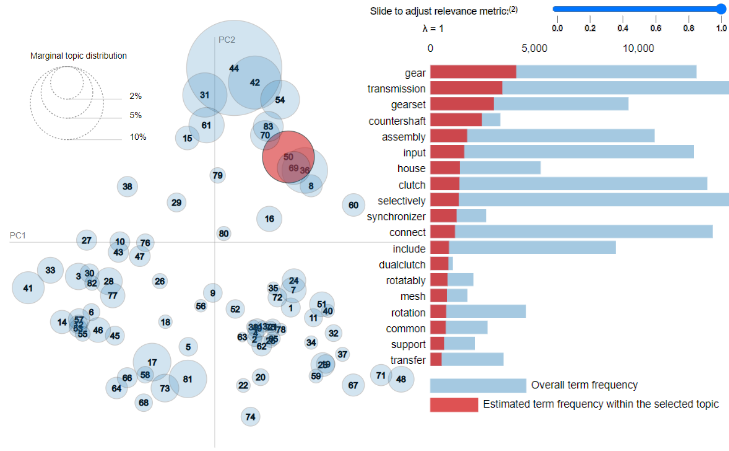
\includegraphics[width=19.29cm,keepaspectratio=true]{img/clustering_process01.png}
	\caption{
		Interthematische Distanz Karte erstellt mit multidimensionaler Skalierung und die relevantesten Terme für das Thema Nummer 50 bei einem $\lambda = 1,0$
	}
	\label{fig:clustering_process01}
 \end{figure}
\end{landscape}

 
 
In Abbildung \ref{fig:clustering_process02} wurde das $\lambda$ von $1,0$ auf $0,6$ herabgesetzt. Dadurch werden die Terme im ausgewählten Thema absteigend nach Relevanz sortiert. Der Parameter $\lambda$ soll mit dem Wert $0,6$ den Anwender die korrektesten  Themen finden lassen \parencite[vgl.][S. 66-68]{sievert2014ldavis}. Rechts wurde der Term \emph{countershaft} ausgewählt. Dadurch werden die Themenradien, abhängig von der Verteilung des ausgewählten Terms, skaliert. Die Themen 50, 20 und 83 enthalten die meisten der \emph{countershaft} Terme und sind teil des pink eingekreisten Subcluster des \emph{transmission} Clusters, aus Abbildung \ref{fig:Themengruppen_LDA_Unigramm}. Deshalb sind sie als \emph{countershaft} Themen zu werten.

\begin{landscape}
	\begin{figure}[htpb]
		\centering
		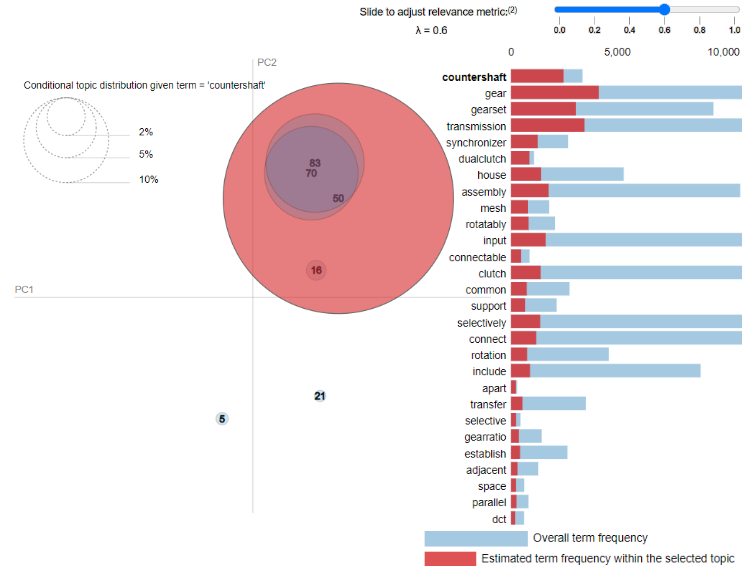
\includegraphics[width=19.29cm,keepaspectratio=true]{img/clustering_process02.png}
		\caption{
			Interthematische Distanz Karte erstellt mit multidimensionaler Skalierung mit einer Themenverteilung welche von dem Term countershaft abhängt und die relevantesten Terme für das Thema Nummer 50 bei einem $\lambda = 0,6$ 
		}
		\label{fig:clustering_process02}
	\end{figure}
\end{landscape}

 
Außerdem kommen die äquivalenten Terme \emph{dualclutch}, \emph{dct} und \emph{automatictransmission} besonders häufig in den Themen 50, 83, 69 und 10 vor. Das ist ein weiterer Teil des Subclusters \emph{transmission}. Des weiteren sind die Terme \emph{synchronizer} und \emph{mesh} beide in den Themen 50, 70 und benachbarten Themen häufig zu finden. Das deutet auf das synchronisieren der \emph{shafts} hin. Durch dieses qualitative Verfahren werden die Themen benannt und Cluster gebildet. Doch \gls{pyLDAvis} reicht allein nicht immer aus. Thema 77 deutet mit den Termen \emph{clutch} und \emph{slip} auf eine Slipper clutch hin aber warum befindet es sich dann in dem \emph{method} Cluster? Für genauere Einblicke in Themen wurde mit \gls{lda} eine Patent-Themen-Matrix erstellt. Das Patent 9,989,146 passt am besten zu Thema 77. Es beschreibt eine Methode, welche den optimalen Druck einer \emph{clutch} in einem \gls{cvt} erlernt, damit die sie einen \emph{pulley slip} verhindern kann. Daher kommt in diesem Thema der Term \emph{pressure} ohne \emph{fluid} oder \emph{hydraulik} vor.
 
 \begin{figure}[htpb]
 	\centering
 	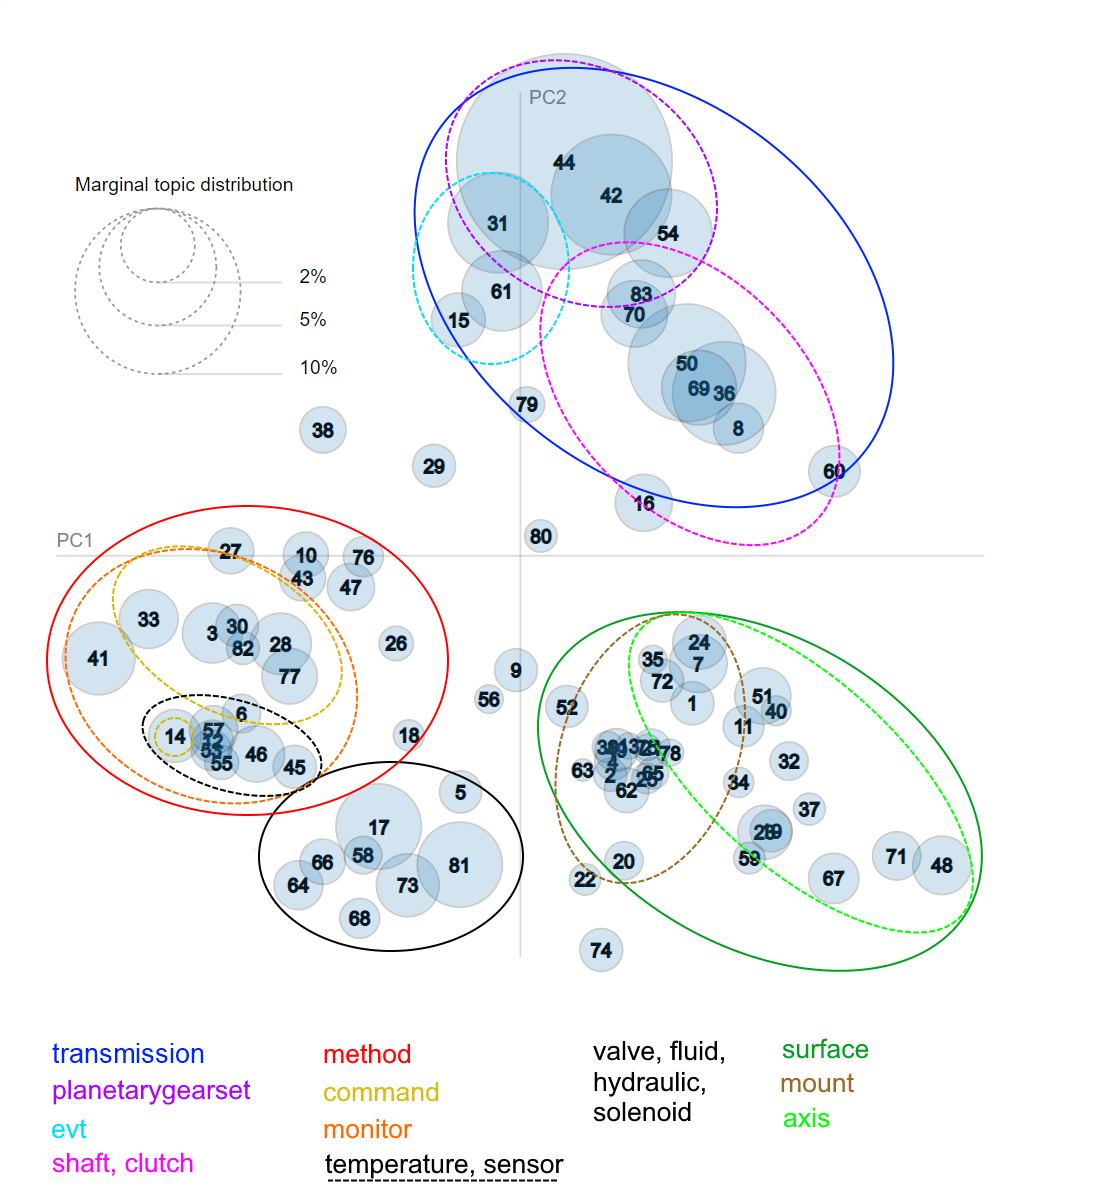
\includegraphics[width=\textwidth,keepaspectratio=true]{img/LDAvisGM-3-1-1_clustered.png}
 	\caption{
 		Themengruppen der LDA Unigramme multidimensionale Skalierung
 	}
 	\label{fig:Themengruppen_LDA_Unigramm}
 \end{figure}
 
 
Der blaue Cluster besteht hauptsächlich aus Themen zu \emph{transmission} Komponenten. Fast alle Themen des blauen Clusters enthalten die Terme \emph{transmission}, \emph{sungear} und \emph{ringgear}. Der lila Subcluster enthält das größte Thema des Datensatzes Nummer 44. Die Themen beinhalten das \emph{planetarygearset}, die \emph{multispeedtransmission} und werden zum \emph{torquetransmit} genutzt. Der türkise Cluster zeigt das Thema \gls{evt} mit einem \emph{motorgenerator} für Hybridautos. Der pinke Cluster beinhaltet die \emph{dualclutch}, die  \emph{automatictransmission}, den \emph{countershaft}, den \emph{inputshaft} und die \emph{synchronizer} welche die \emph{shafts} verbinden (\emph{mesh}). Dies wird im Patent 8,240,224 beschrieben.
 
Der Rote Cluster enthält besonders viele Terme wie \emph{method}, \emph{command} und \emph{request}. Der Cluster besteht daher aus Steuerungs- und Regelungsthemen von Fahrzeugen.
 
Im gelben Subcluster geht es hauptsächlich um die elektronische Steuerung von Kupplungen, dem Motor und dem \gls{cvt}. Er ist eine Teilmenge des orangen Subclusters, weil in dem gelben Subcluster viel häufiger der Term \emph{command} vorkommt und \emph{montior} gleichmäßiger im gesamten orangen Subcluster einschließlich des gelben Subclusters verteilt ist. Das Thema Nummer 14 ist eine Ausnahme, weil es fast gleich viele Terme von \emph{command} und \emph{monitor} für die \emph{hydraulic} \emph{pressure} enthält. Deshalb ist es extra gelb umkreist. Die \emph{frictionclutch} ist hauptsächlich dem Thema 77 zuzuordnen. Der Term \emph{slip} kommt in Verbindung mit der \emph{clutch} in den umliegenden Themen häufig vor. Auch die \emph{dogclutch} ist in dem gelben Subcluster zu finden obwohl sie hauptsächlich im Thema 5 vorkommt. Im Thema 28 geht es um die Steuerung der \emph{binary} \emph{clutch} (9,061,675), die im Thema 50 schon \emph{dualclutch} genannt wurde. Das Thema 3 umfasst das besagte \gls{cvt}. Fast alle Themen des roten Clusters sind eng verbunden mit dem \emph{engine}, besonders die Themen 41 und 33.
 
Der schwarze Subcluster enthält viele Themen zur Beobachtung (\emph{monitor}, \emph{sensor}) der \emph{temperature} und der \emph{pressure}. In diesem schwarzen Subcluster geht es hauptsächlich um Themen die mit Flüssigkeit in Verbindung stehen. Es geht um die \emph{hydraulic} \emph{pressure} (14), die \emph{hydraulic} \emph{pump} (45) und die \emph{temperature} des \emph{coolant} im Kühlkreislauf der \emph{electricmachine} (8,167,773), der \emph{engine} und des \emph{radiator} (57). Durch die Steuerung des Kühlkreislauf können Komponenten wie die \emph{transmission} auf Betriebstemperatur gebracht werden (10,161,501). Zu dem Thema 12 passt am besten das Patent 9,404,403, es beschreibt eine Methode um das Öllevel zu beobachten (\emph{monitor}). Auf Grund der vielen Flüssigkeitsthemen befindet sich der schwarze Subcluster in der Nähe des schwarzen Hauptclusters.
 
Der schwarze Hauptcluster enthält fast alle Themen die in Verbindung mit Flüssigkeit stehen. Er teilt die Häufigkeit des von \emph{control} mit dem roten Cluster aber unterscheidet sich durch die Verwendung von die Terme \emph{communication} und \emph{communicate} die sonst nur selten auftreten. Besonders häufig ist die Kombination \emph{solenoid}, \emph{hydraulic}, \emph{valve} und \emph{fluid}. Das Thema 17 beschreibt in mehreren Patenten (8,820,185
, 8,382,639) die Steuerung einer \emph{dualclutch} mithilfe von \emph{hydraulic} und \emph{solenoids}. Mit einem Elekrtomagnet (\emph{solenoids}) wird ein Verschluss aus der \emph{valve} gezogen. Dieser Verschluss wird nach dem nach dem Ausschalten des \emph{solenoids} mit einer Feder zurück in die \emph{valve} geschoben. Mit einem \emph{solenoid} kann auch Druck erzeugt werden. Daher kommt der Term \emph{pressure} ebenfalls häufig vor. Diese Methode findet Verwendung in Thema 68, dort wird beschrieben wie eine \emph{actuator} \emph{fork} kontrolliert (\emph{control}) werden kann (9,605,755).

Der dunkel grüne Cluster besteht aus sehr vielen kleinen Themen die nicht gänzlich durch thematische Nähe gruppiert wurden. Ein gemeinsamer Term ist \emph{bias} was auf Zahnräder hindeutet. Das ist leider unspezifisch. Der hellgrüne Subcluster hingegen hat zwei beschreibende Terme. \emph{shaft}, \emph{axis} und \emph{house} zeigen eine Verwandschaft mit dem pinken Subcluster, der ebenfalls \emph{shaft} \emph{house} enthält. Das \emph{house} deutet auf das gear housing hin was auch zu den Termen \emph{surface}, \emph{side} und \emph{body} passt die den gesamten dunkelgrünen Cluster bilden.
 
 
%\todo[inline]{DVU, TCM, ECM, VSR, DCT, ETR? gelber cluster}
 
%Der orange Subcluster 
 
 
 
%9 layshaft
%52 turbine
 
 


\section{Analyse der Ergebnisse des \gls{hlda}}

Die Ergebnisse des \gls{hlda} werden im Vergleich mit den \gls{lda} Ergebnissen analysiert. Zwei Subcluster des \gls{hlda} Baums werden mit den Ergebnissen des \gls{lda} verglichen und analysiert. Der ganze \gls{hlda} Baum ist zu groß um leserlich abgebildet zu werden. Er kann im digitalen Anhang mit einem Programm geöffnet werden, das graphml unterstützt, zum Beispiel Cytoscape.

Der \emph{engine} Subcluster aus Abbildung \ref{fig:hlda_engine} passt gut zu dem orangefarbenen Subcluster aus der \gls{lda} Abbildung \ref{fig:Themengruppen_LDA_Unigramm}. Die Terme \emph{engine} und \emph{fuel} passen zu dem Motorthema 41. Die Subthema \emph{monitor} passt genau zu dem orangefarbenen Subcluster und \emph{temperature} gehört mit \emph{electricmachine} zum Thema 57. Dadurch werden die mit \gls{lda} benannten Themen bestätigt. Die Subthemen \emph{operate}, \emph{shift} und \emph{drum} sind im \gls{lda} Modell in dieser Form nicht in der Nähe aufzufinden. Allerdings passen sie thematisch zu den anderen.

\begin{figure}[htpb]
	\centering
	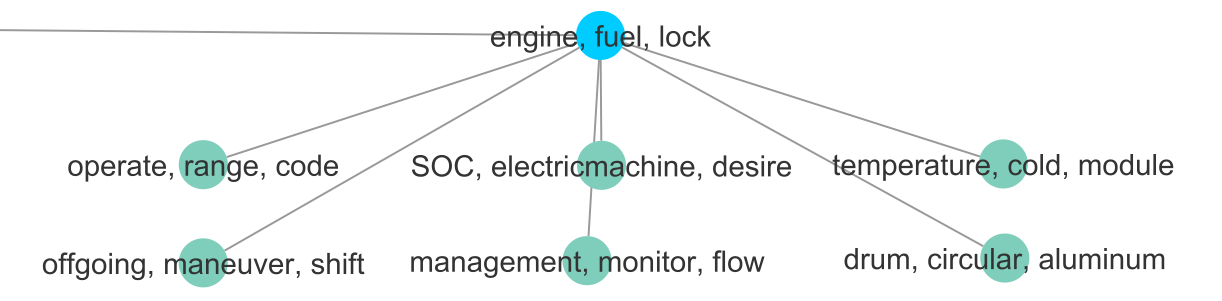
\includegraphics[width=\textwidth,keepaspectratio=true]{img/hldaEngine.png}
	\caption{
		Der \emph{engine} Ausschnitt des \gls{hlda} Baums
	}
	\label{fig:hlda_engine}
\end{figure}

Der \emph{fork} Subcluster aus Abbildung \ref{fig:hlda_fork} passt genau zu dem schwarzen Cluster aus Abbildung \ref{fig:Themengruppen_LDA_Unigramm}. Dort beschreibt das Thema 68 ebenfalls eine \emph{synchronizer actuator fork} aus dem Patent 9,605,755. Der \gls{hlda} Subcluster enthält außerdem die Subthemen \emph{valve}, \emph{spool}, \emph{cool}, \emph{pressure}, \emph{calibrate}, \emph{position} und \emph{control}. Diese kommen auch alle im \gls{lda} Cluster vor und bestätigen erneut die Ergebnisse. Die \emph{spool} ist eine Spule und daher ein Bestandteil des Elektromagneten \emph{solenoid}.

\begin{figure}[htpb]
	\centering
	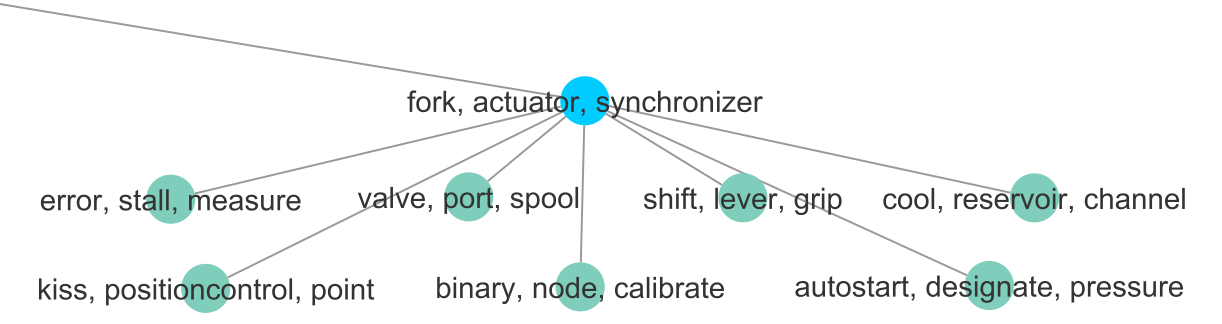
\includegraphics[width=\textwidth,keepaspectratio=true]{img/hldaFork.png}
	\caption{
		Der \emph{fork} Ausschnitt des \gls{hlda} Baums
	}
	\label{fig:hlda_fork}
\end{figure}


\section{Analyse der Ergebnisse des \gls{dlda}}

Die Ergebnisse des \gls{dlda} werden zuerst eingeordnet und die Wahl der Terme, welche die ausgewählten Cluster und Themen repräsentieren, erläutert. Dann werden die Trends der Terme festgestellt.

Der \gls{dlda} wurde mit den Ergebnissen des \gls{lda} und den Anmeldedaten der Patente gespeist. Daher sind die Ergebnisse des \gls{dlda} direkt vergleichbar mit denen des \gls{lda}. Die Terme wurden so gewählt, dass sie die Cluster möglichst genau beschreiben. Außerdem sollen sie relativ selten in anderen Clustern vorkommen, damit ihr Trend nicht verfälscht wird. Diese Bedingungen der Clusterbenennung wurden in \ref{lda_analysis} berücksichtigt.



  \begin{figure}[!ht]
	\centering
	\begin{floatrow}
		\ffigbox[\FBwidth]{\caption{Trends der Terme die ihren Cluster am besten beschreiben}\label{fig:dlda_overall}}{%
			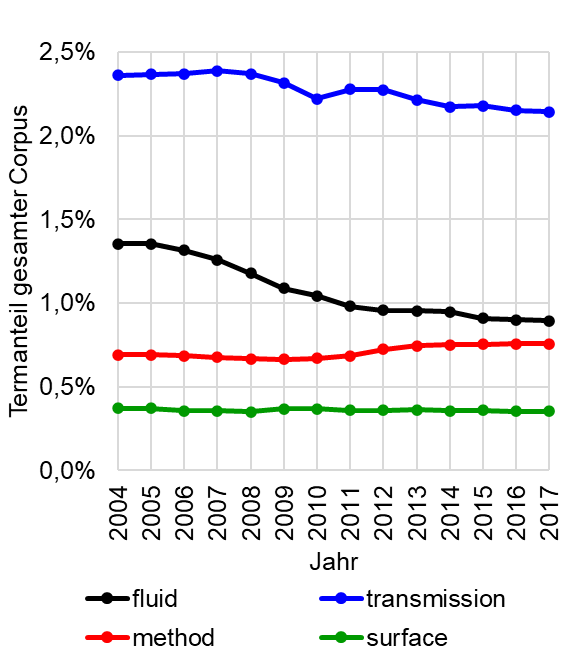
\includegraphics[width=\linewidth,keepaspectratio=true]{img/DLDA_overall.png}
		}
		\ffigbox[\FBwidth]{\caption{Trends der 3 Terme die das Thema 50 am besten beschreiben}\label{fig:dlda_topic_50}}{%
			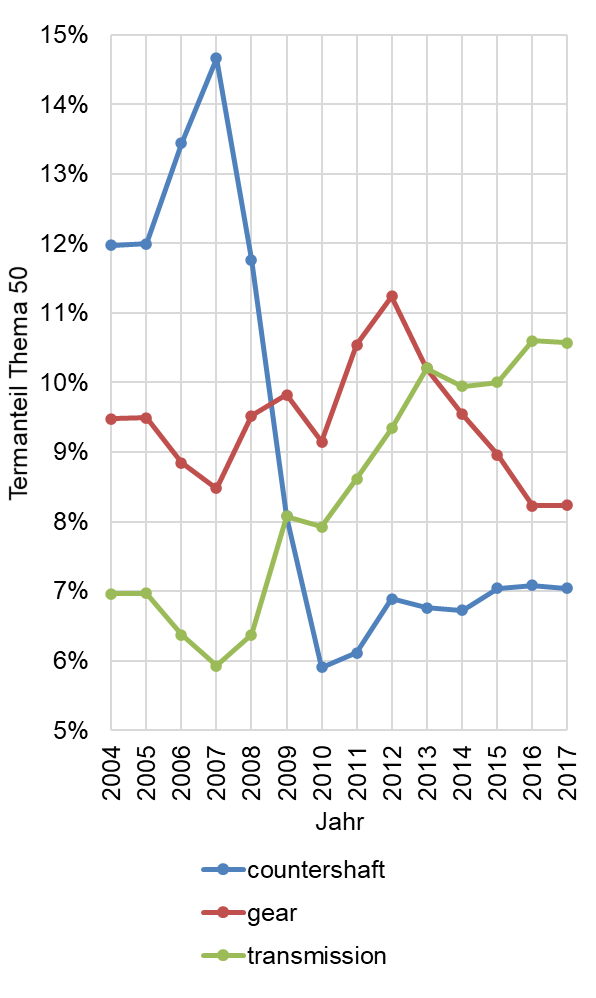
\includegraphics[width=\linewidth,keepaspectratio=true]{img/DLDA_topic_50.png}
		}
	\end{floatrow}
\end{figure}


\section{Vergleich der Ergebnisse anhand von Kennzahlen}
Die Unigrammmodelle weisen eine niedrigere Distanz zueinander auf als die Bigrammmodelle. Das liegt daran, das es deutlich mehr Bigramme gibt und diese auch als unterschiedlich gewertet werden wenn sie sich nur teilweise unterscheiden. Ein Beispiel wäre gear gearset und gear gear. In \ref{fig:Kohärenz_Distanz_Unigramme} wird ersichtlich das sich die Kohärenz mit steigender Themenzahl verbessert bis sie gleich der Anzahl an Wörtern im Datensatz ist. Die Distanz hingegen sinkt nachdem sie einen Hochpunkt erreicht. In Abbildung 4.1 sind Muster und Hotspots aus Unigrammthemen zu erkennen, die besonders ähnlich oder unähnlich sind. Diese werden später geclustered. In Abbildung 4.2 gibt es ebenfalls Muster und Hotspots. Allerdings sind manche Bigrammthemen disjunkt, wodurch sie eine Distanz von 1 haben. 

\begin{table}
	\RawFloats
	\centering
	\caption{Kohärenzen}
	\begin{tabular}{|c|c|c|}
		\hline
		Modell & Unigramm & Bigramm \\
		\hline
		LDA & -2,03 & -5,51 \\
		\hline
		HLDA & -4,30 & -5,90 \\
		\hline
	\end{tabular}
	\label{table:Kohärenzen}
\end{table} 

\begin{figure}[htpb]
	\centering
	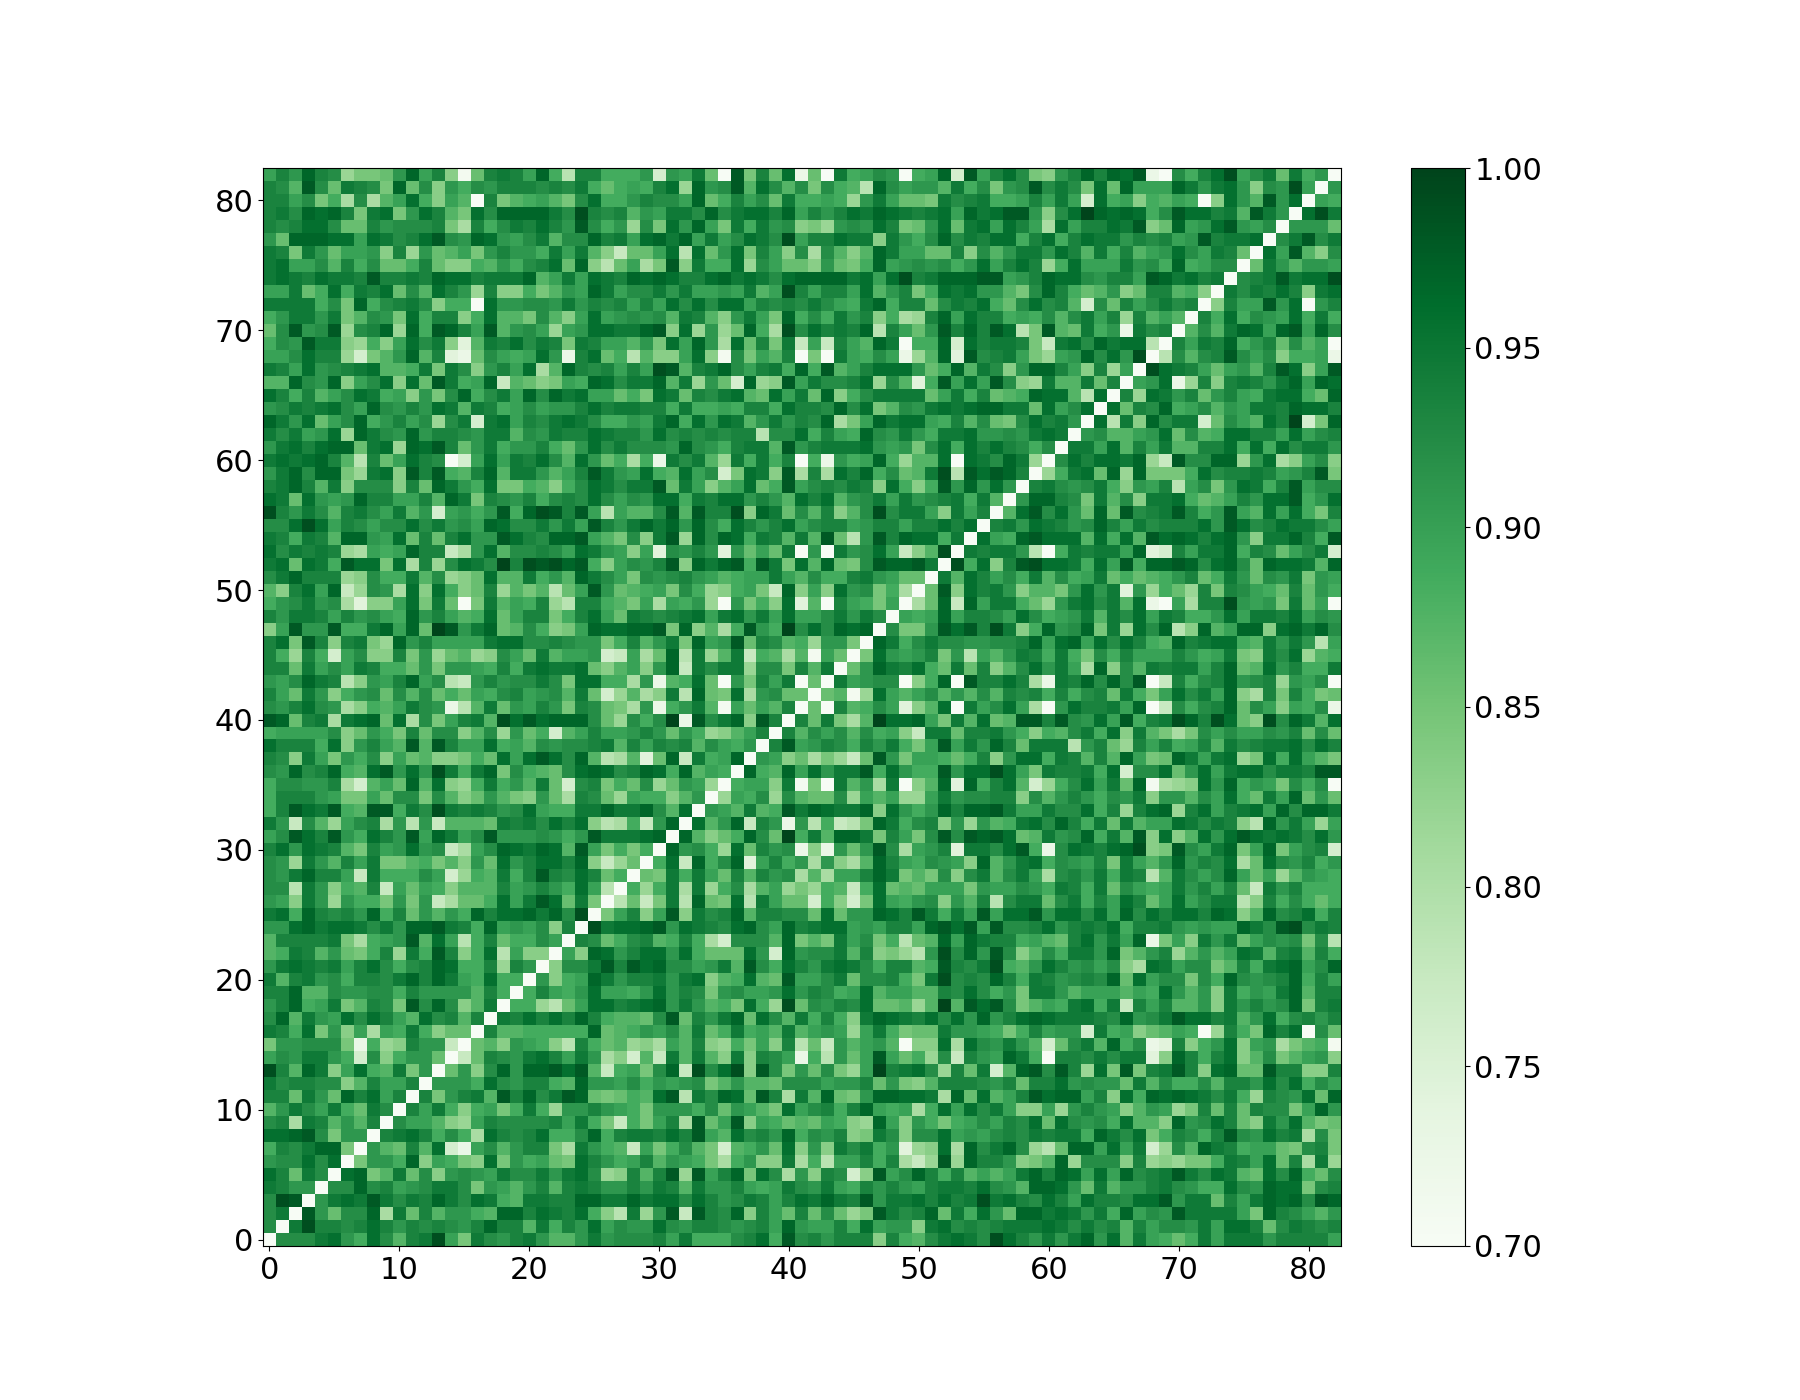
\includegraphics[width=\textwidth,height=12cm,keepaspectratio=true]{img/unigram_jaccard_50_green_07.png}
	\caption{
		Distanz zwischen den top 50 Unigrammen der Themen
	}
	\label{fig:Distanz_Unigramme}
\end{figure}

\begin{figure}[htpb]
	\centering
	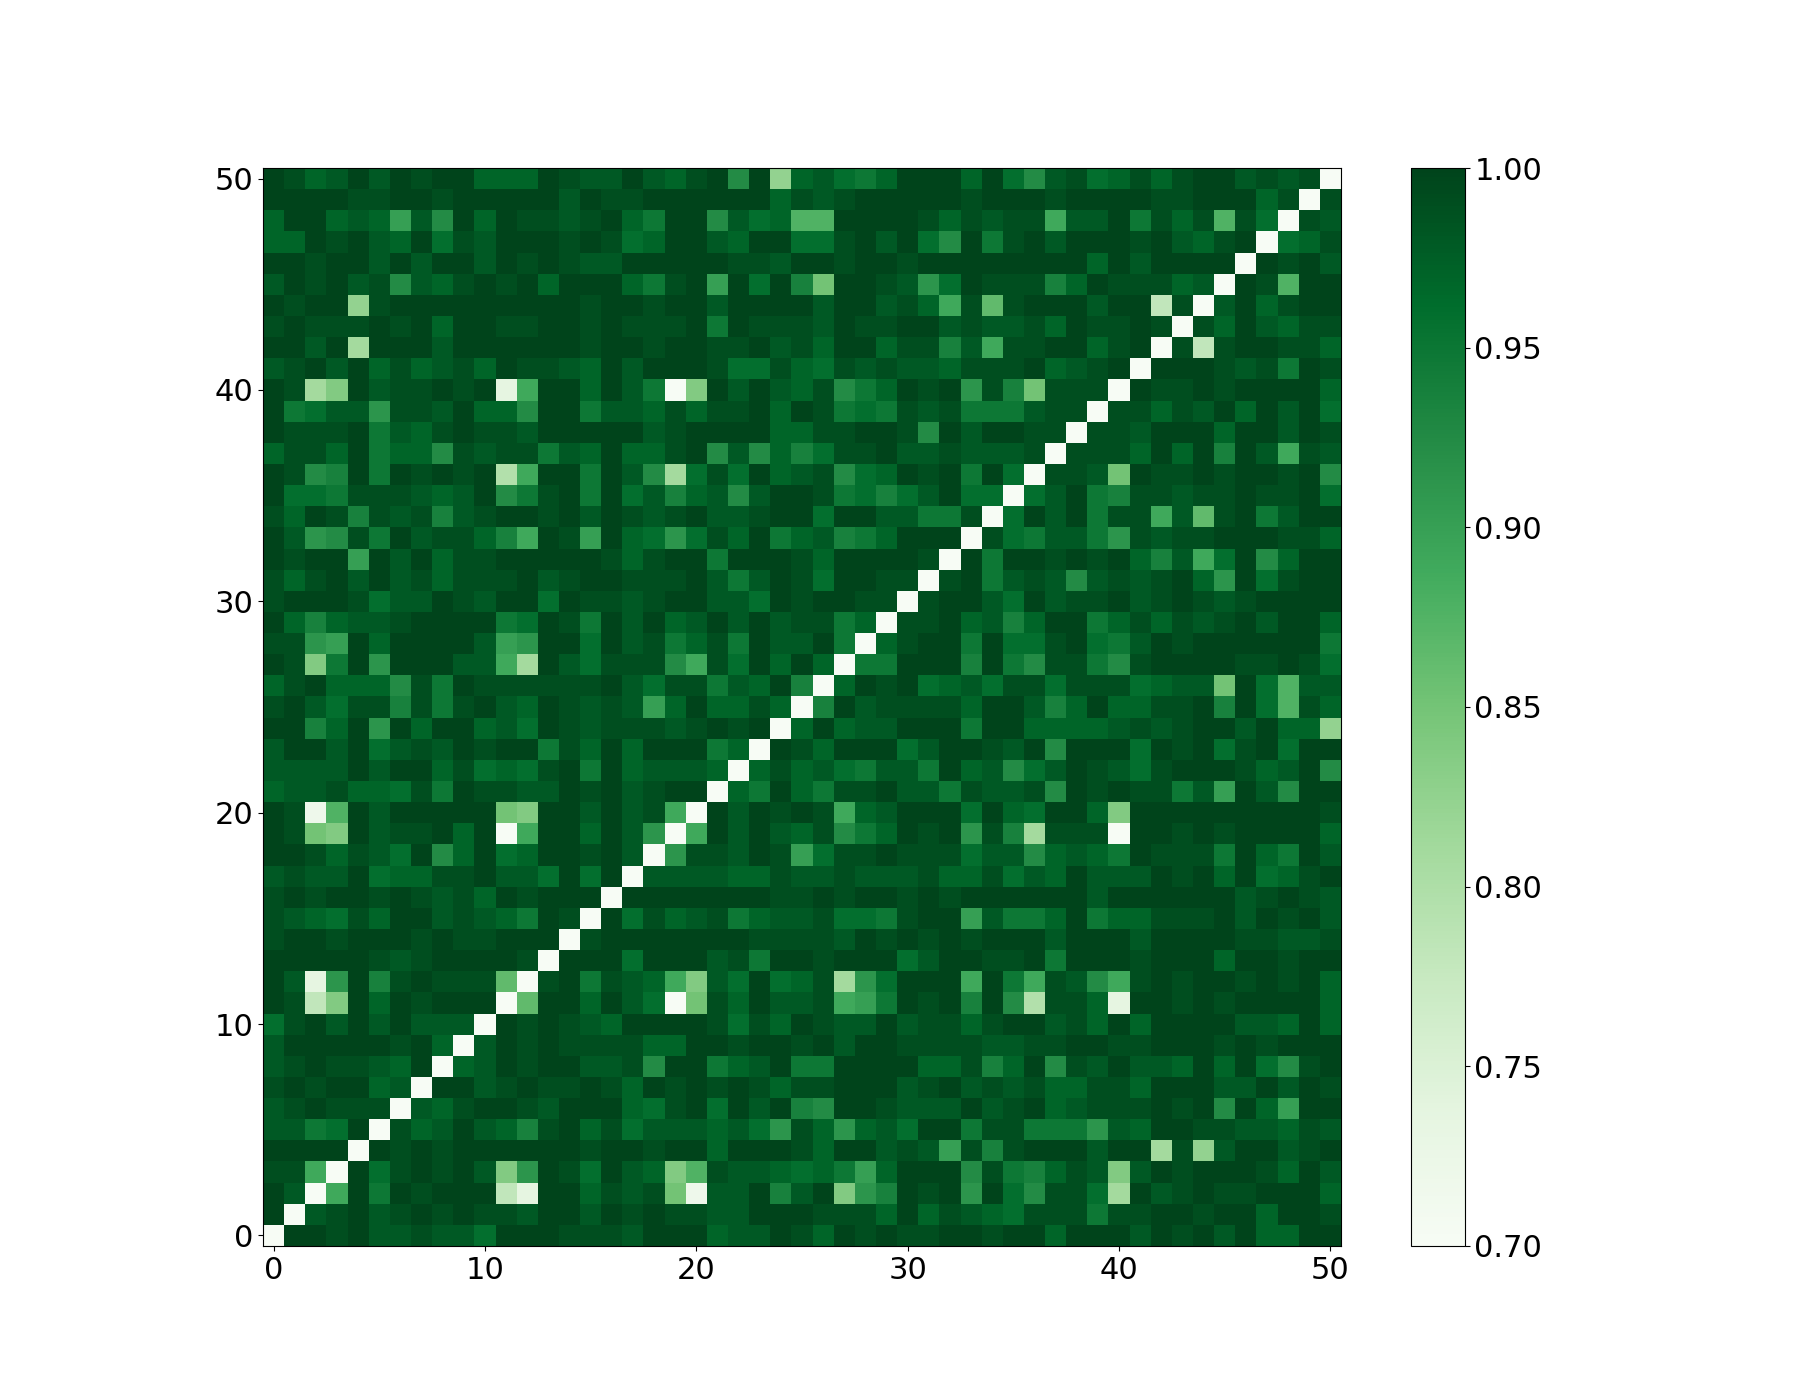
\includegraphics[width=\textwidth,height=12cm,keepaspectratio=true]{img/bigram_jaccard_50_green_07.png}
	\caption{
		Distanz zwischen den top 50 Bigrammen der Themen
	}
	\label{fig:Distanz_Bigramme}
\end{figure}